\documentclass[10pt,twocolumn]{article}

%%% packages %%%
\usepackage{color}
\usepackage{graphicx}
\usepackage{listings}
\usepackage{float}
\usepackage{url}
\usepackage{times}
\usepackage{xspace}
\usepackage{microtype}
\begin{document}

\title{Finding Dominators\ \\
  \small CSE 501 Spring 2013 Compilers Assignment 1}
\author{Andre Baixo, Jacob Nelson}
\maketitle

This writeup describes our optimizer implmentation for Assignment 1.

\section{Implementation}

Our optimizer implements the dominance algorithm described in~\cite{Cooper_asimple}. 

Programs are processed in four phases. In the first phase, we parse
the textual representation of the intermediate language output from
the Start front-end and create an object for each element
found. Non-executable elements like the {\it method} construct are
stored separately from the executable instructions.

In the second phase, we form the instructions into basic blocks. To do
this, we use the {\it method} elements in the input to partition the
set of instructions; then we iterate over the instructions in each
method's set and divide them into basic blocks based on branch (and
other) instructions as well as branch targets.

In the third phase, we form the control flow graph by adding edges
between the basic blocks based on program order as well as branch
targets. We store both successor and predecessor edges to make
traversal cheaper.

Finally, we compute dominators for each method. The first step here is
to compute a topological order over the basic blocks in the method. We
do this by running a depth-first search over the CFG. Once we have
that order, we execute the dominance algorithm, iteratively refining
each block's immmediate dominator until nothing changes. When that is
complete, we store the immediate dominators in the blocks and add the
dominator tree edges to the CFG.


\section{Examples}

\begin{figure}
\begin{center}
  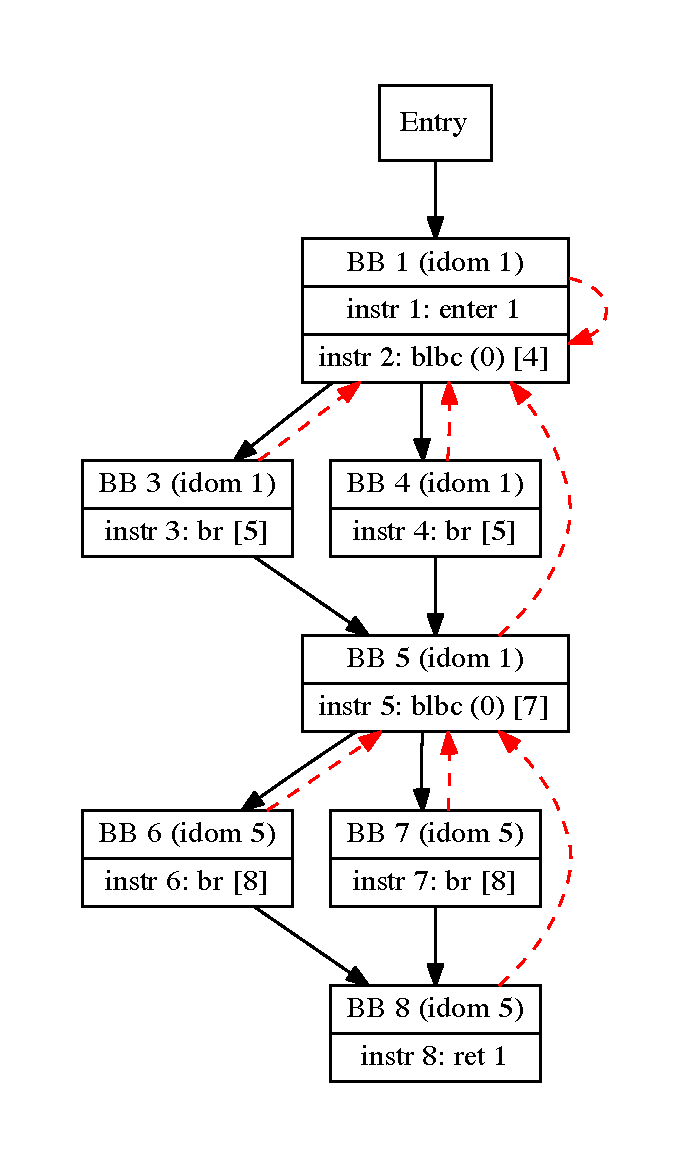
\includegraphics[width=0.95\columnwidth]{figs/hammock.pdf}
\begin{minipage}{0.95\columnwidth}
  \caption{\label{fig:hammock} CFG from hammock example. Red edges show dominator relationships.}
\end{minipage}
\end{center}
\end{figure}

\begin{figure}
\begin{center}
  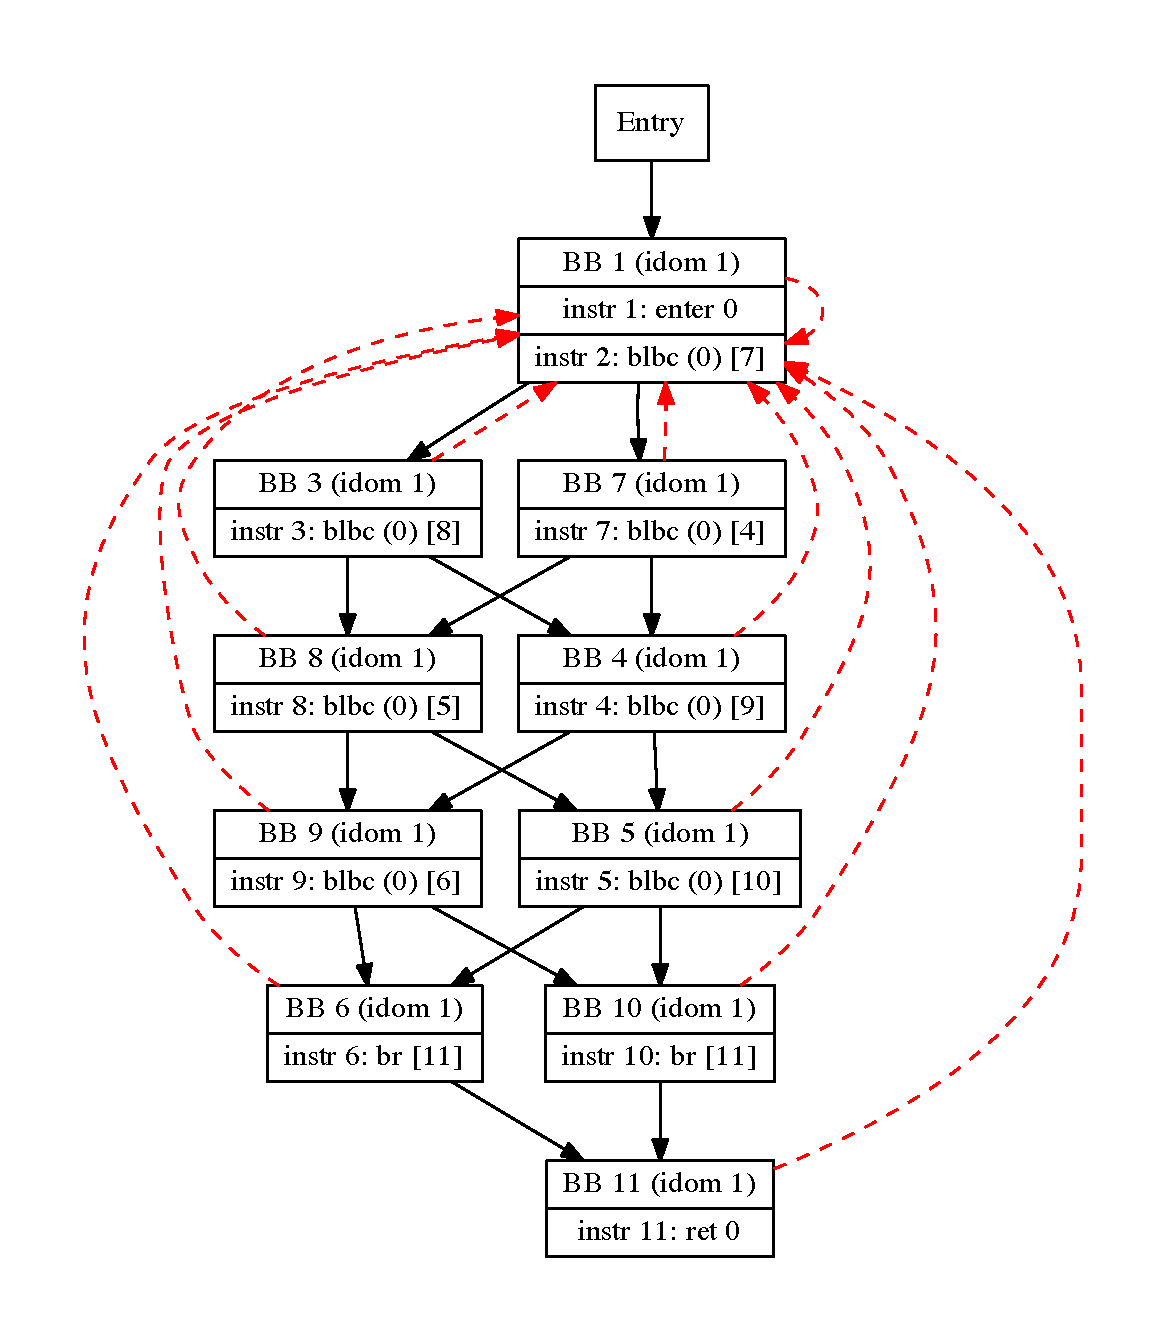
\includegraphics[width=0.95\columnwidth]{figs/weave.pdf}
\begin{minipage}{0.95\columnwidth}
  \caption{\label{fig:weave} CFG from weave example. Red edges show dominator relationships.}
\end{minipage}
\end{center}
\end{figure}

\begin{figure}
\begin{center}
  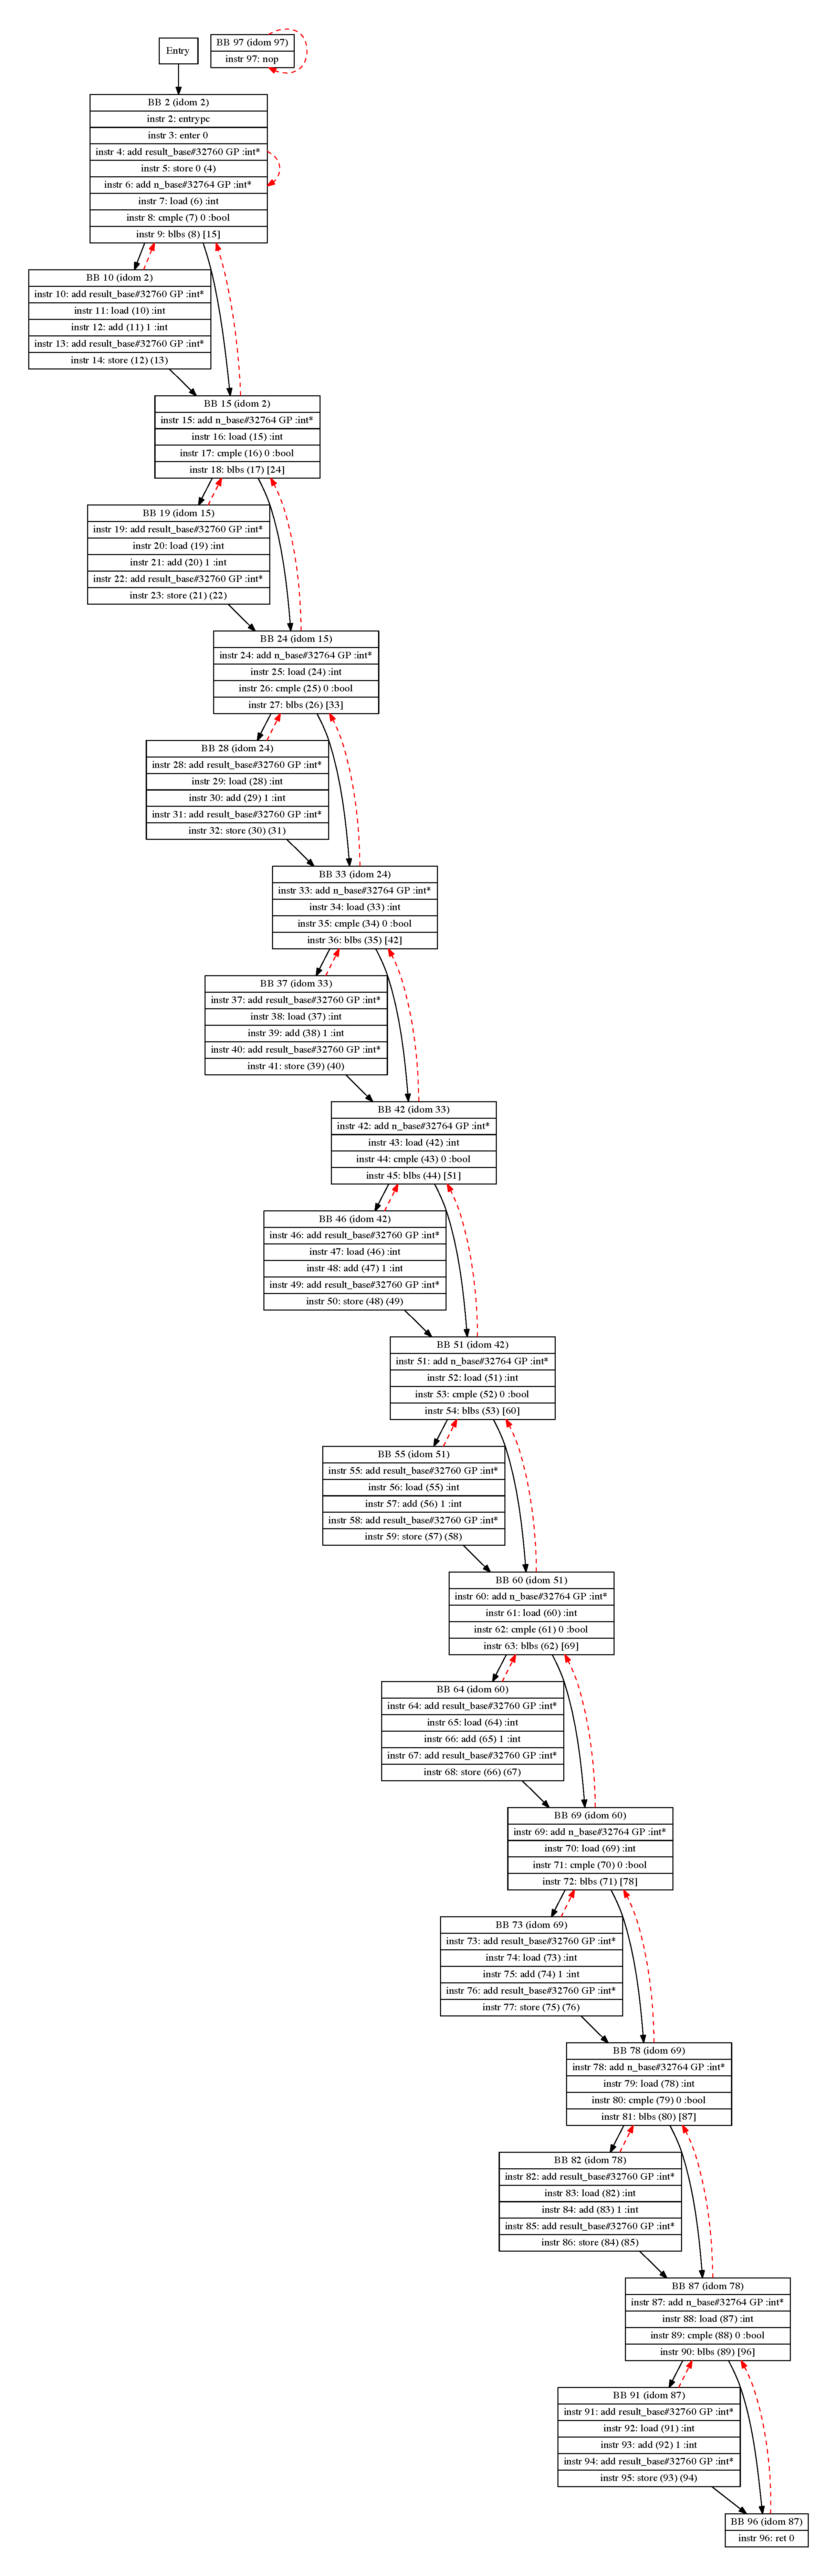
\includegraphics[height=6in]{figs/nested-if-10-1.pdf}
  \caption{CFG from 10-if singly-nested example. Red edges show dominator relationships.}
  \label{fig:nest-10-1}
\end{center}
\end{figure}

\begin{figure}
\begin{center}
  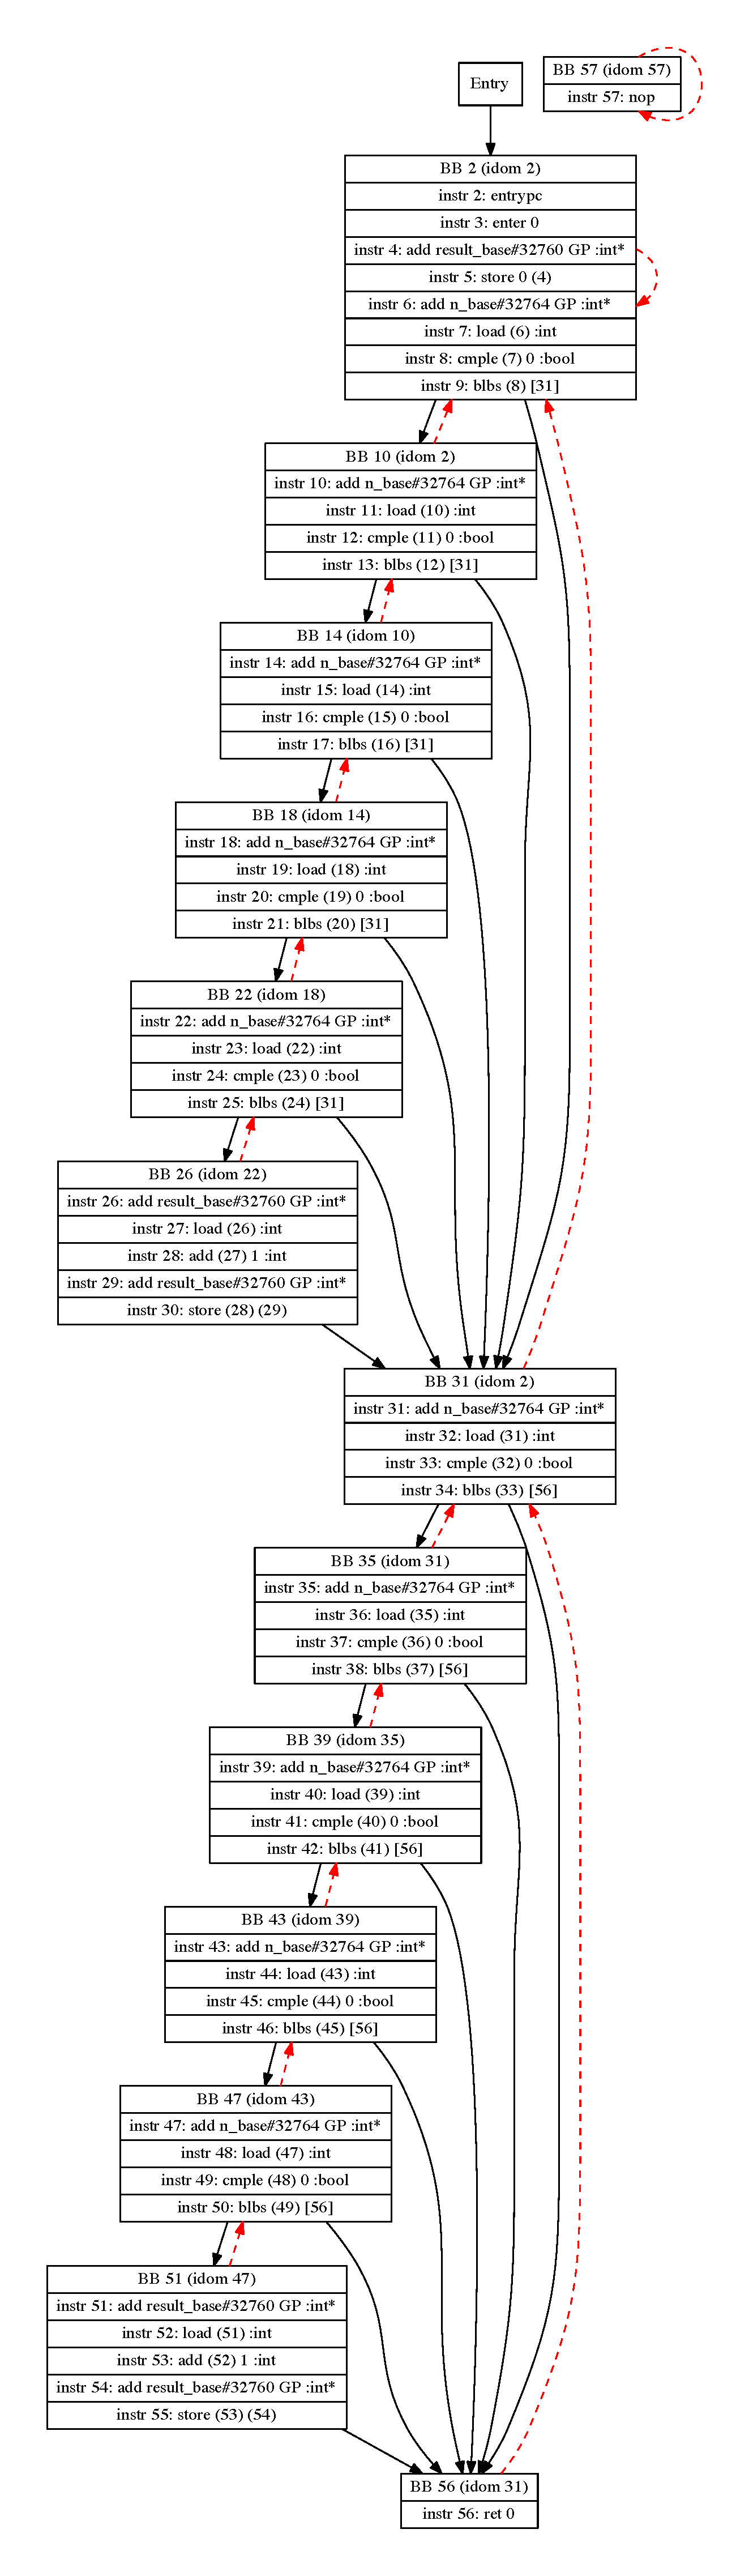
\includegraphics[height=6in]{figs/nested-if-10-5.pdf}
  \caption{CFG from 10-if 5-nested example. Red edges show dominator relationships.}
  \label{fig:nest-10-5} 
\end{center}
\end{figure}

\begin{figure}
\begin{center}
  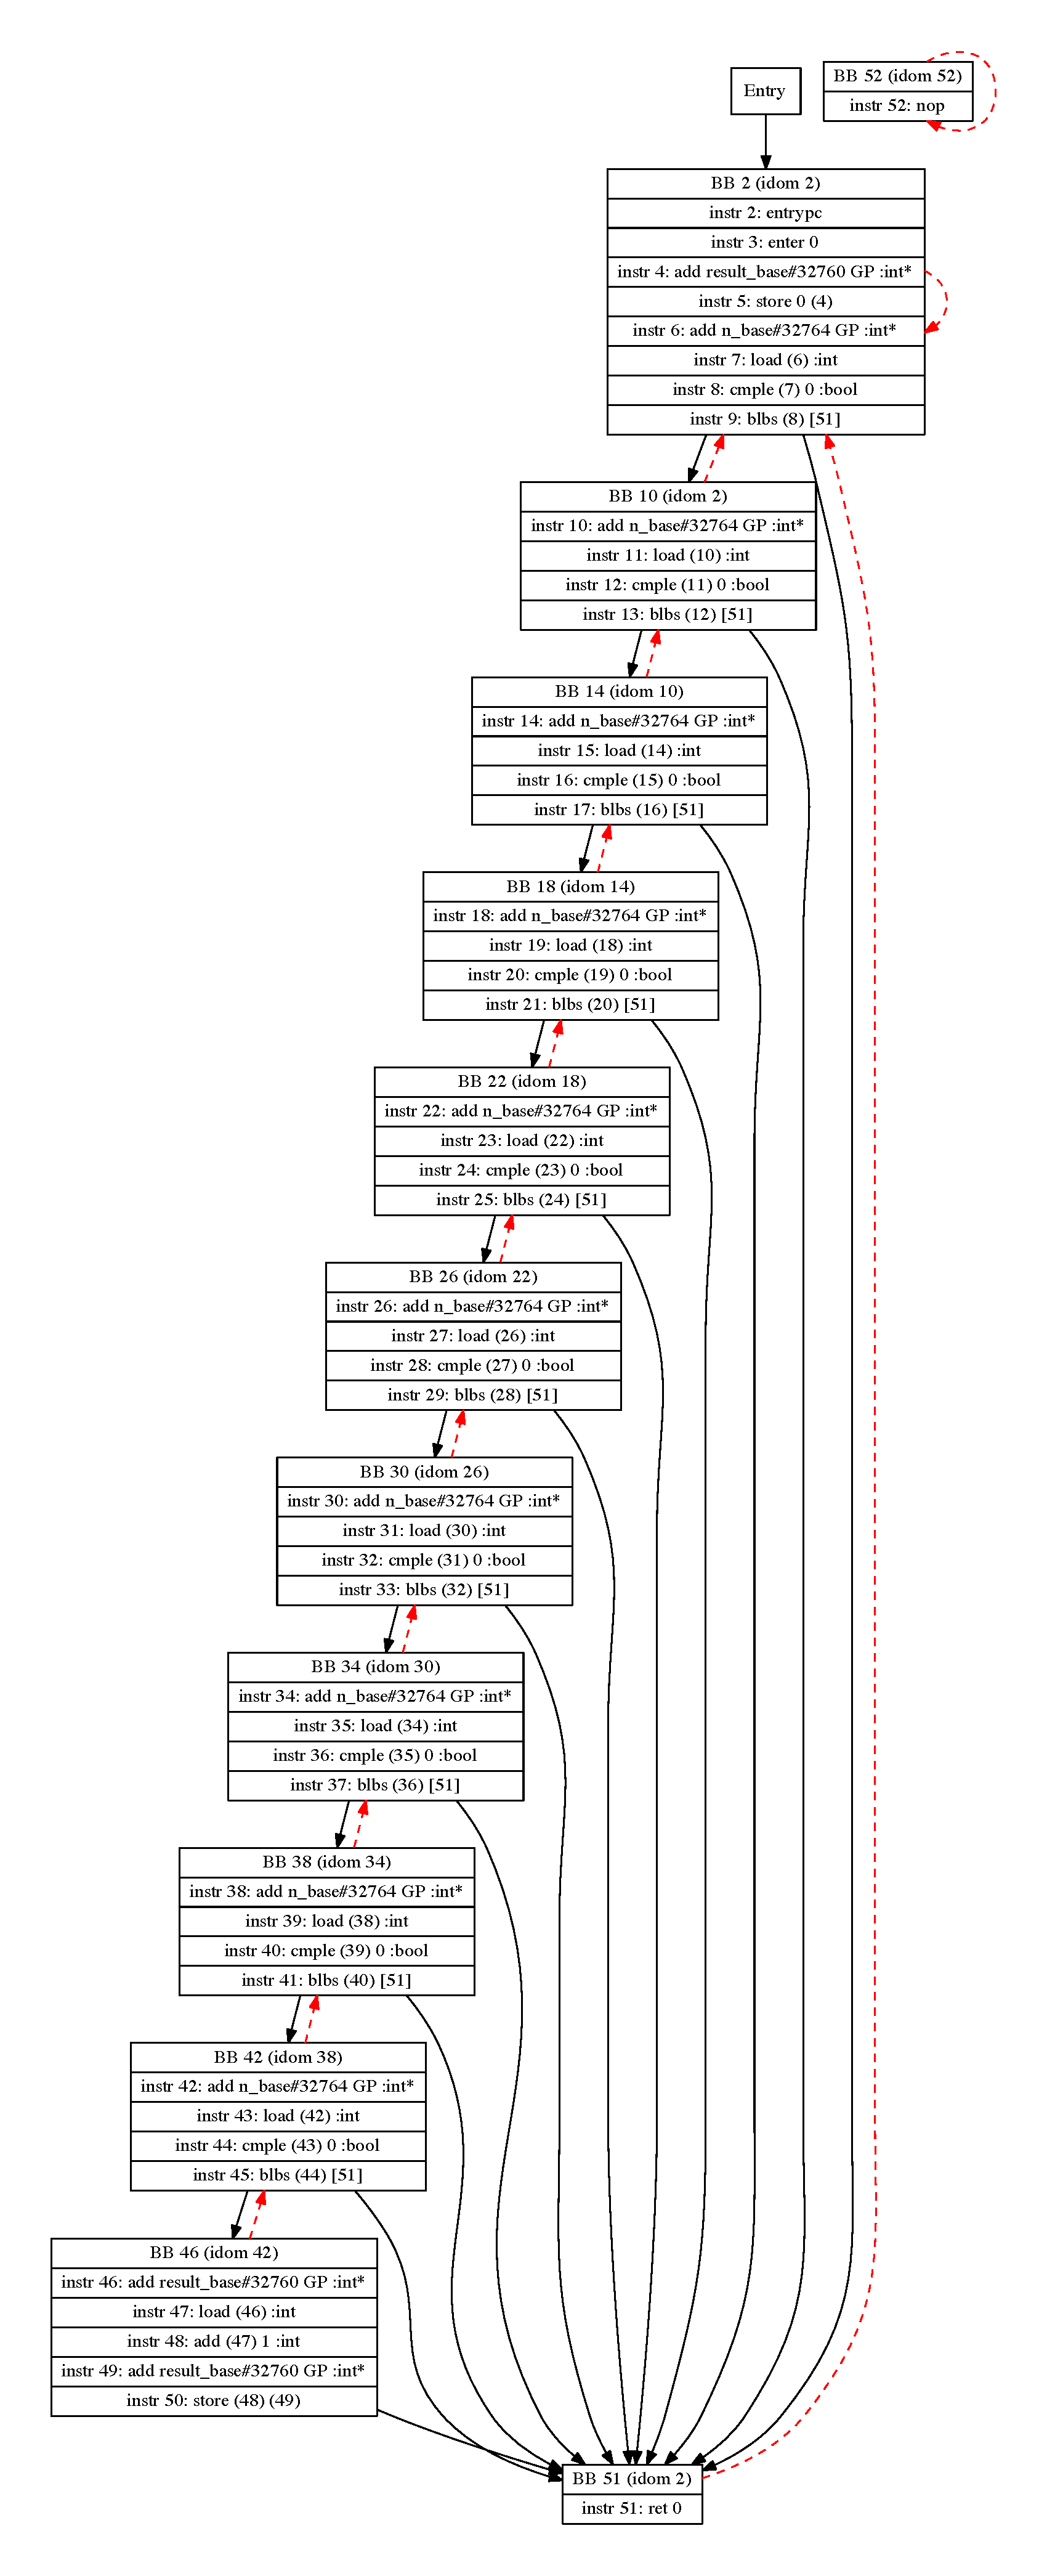
\includegraphics[height=6in]{figs/nested-if-10-10.pdf}
  \caption{CFG from 10-if 10-nested example. Red edges show dominator relationships.}
  \label{fig:nest-10-10} 
\end{center}
\end{figure}

We implemented three additional examples to better understand our
implementation. The first is \texttt{examples/hammock.il}, a simple
dual hammock shown in Figure~\ref{fig:hammock}. The second is
\texttt{examples/weave.il}, a more complicated set of woven branches
shown in Figure~\ref{fig:weave}. Both of these examples provide a simple
verification of our dominator construction.

The third example is a script that generates nested if constructs of
different sizes. The Ruby file \texttt{examples/nested-if.rb} takes
two parameters: a total if-construct count, and a nesting depth. The
nesting depth controls how many levels of nested if constructs are
generated.  Figure~\ref{fig:nest-10-1} shows a CFG from a 10-node,
singly-nested example; figure~\ref{fig:nest-10-5} shows a 10-node,
5-nested example, and figure~\ref{fig:nest-10-10} shows a 10-node,
10-nested example. This lets us explore how the structure of the CFG
affects runtime.

\section{Results}

We explored the performance of our implementation in three ways. For
all our experiments, we ran on an Ivy Bridge-based MacBook Air with
8GB of RAM.

First, we processed all the example programs provided. The
longest-running method was the main method from \texttt{mmm.dart},
which ran for about 200 microseconds. Other data can be generated by
running the \texttt{assignment1/run.sh} script.

Since this time is too short to make meaningful comparisons, we then
used our nested-if generator to create a set of larger programs with
different CFG shapes. Unfortunately we were hampered by our
implementation choices: by depending on the Ruby VM stack for
computing a topological order, we were limited to CFGs whose depth was
on the order of 2000 nodes. This could be easily avoided by modifying
the code to use an external stack for the traversal, but since we
expect that real programs are rarely nested this deep, we chose not to
do this.


\begin{figure}
\begin{center}
  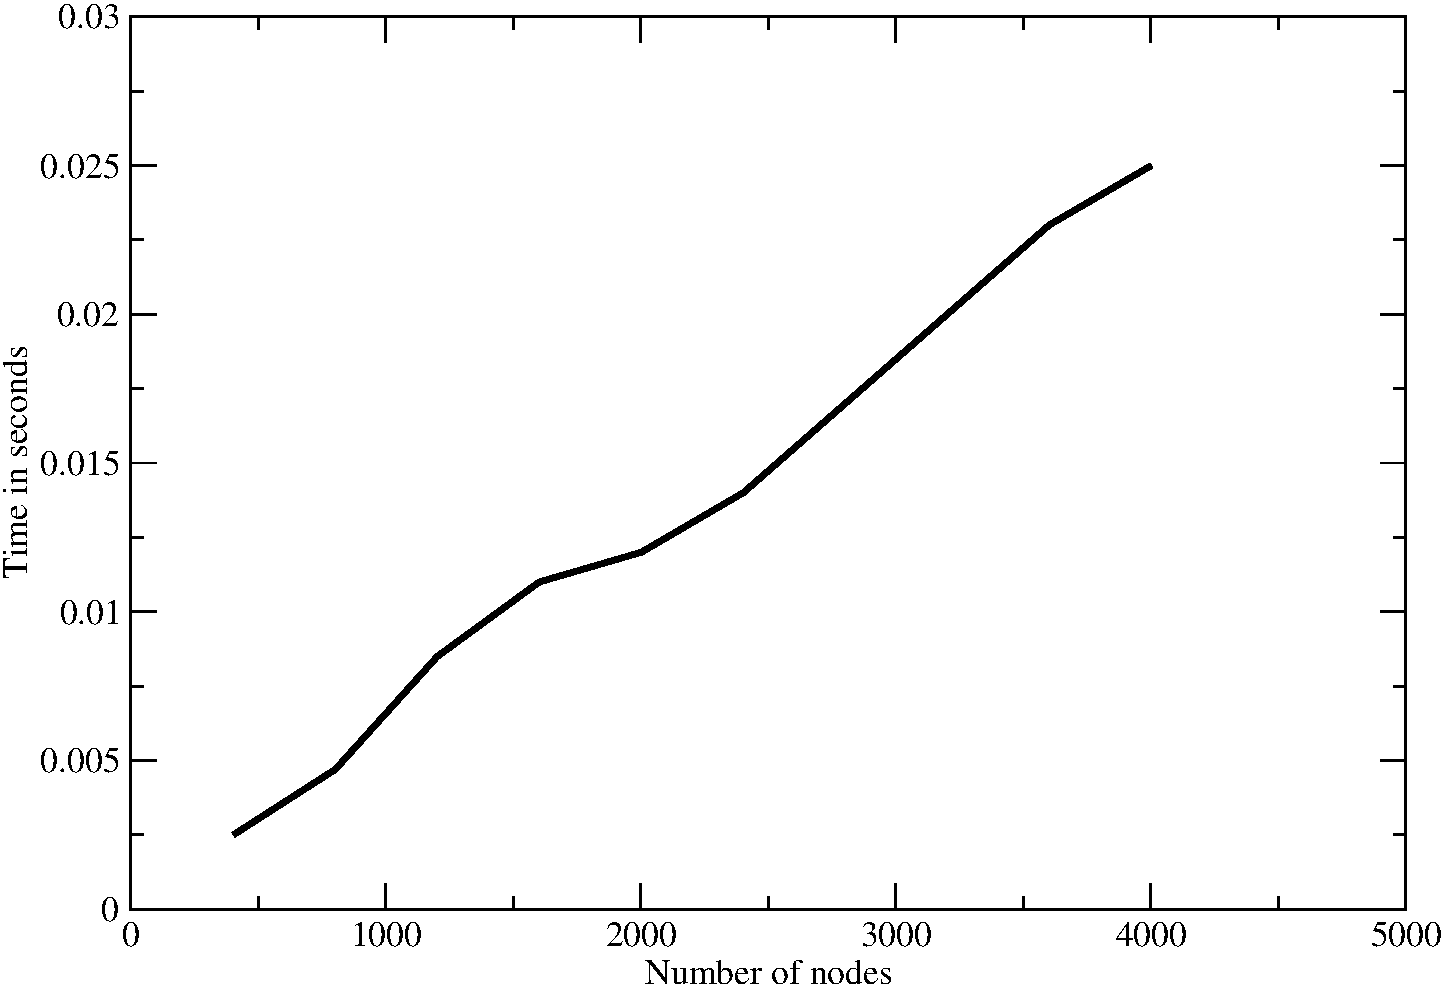
\includegraphics[width=0.95\columnwidth]{figs/g1.pdf}
\begin{minipage}{0.95\columnwidth}
  \caption{\label{fig:nodes} Relationship between CFG node count and runtime in nested if example with nesting depth of 1.}
\end{minipage}
\end{center}
\end{figure}

The first experiment we ran with the nested if generator was intended
to show the cost of scaling the size of the CFG. In this experiment,
we varied the number of nodes and edges together while keeping the
nesting depth fixed at 1. Figure~\ref{fig:nodes} shows the result. We
find that runtime varies linearly with the number of nodes and edges.


\begin{figure}
\begin{center}
  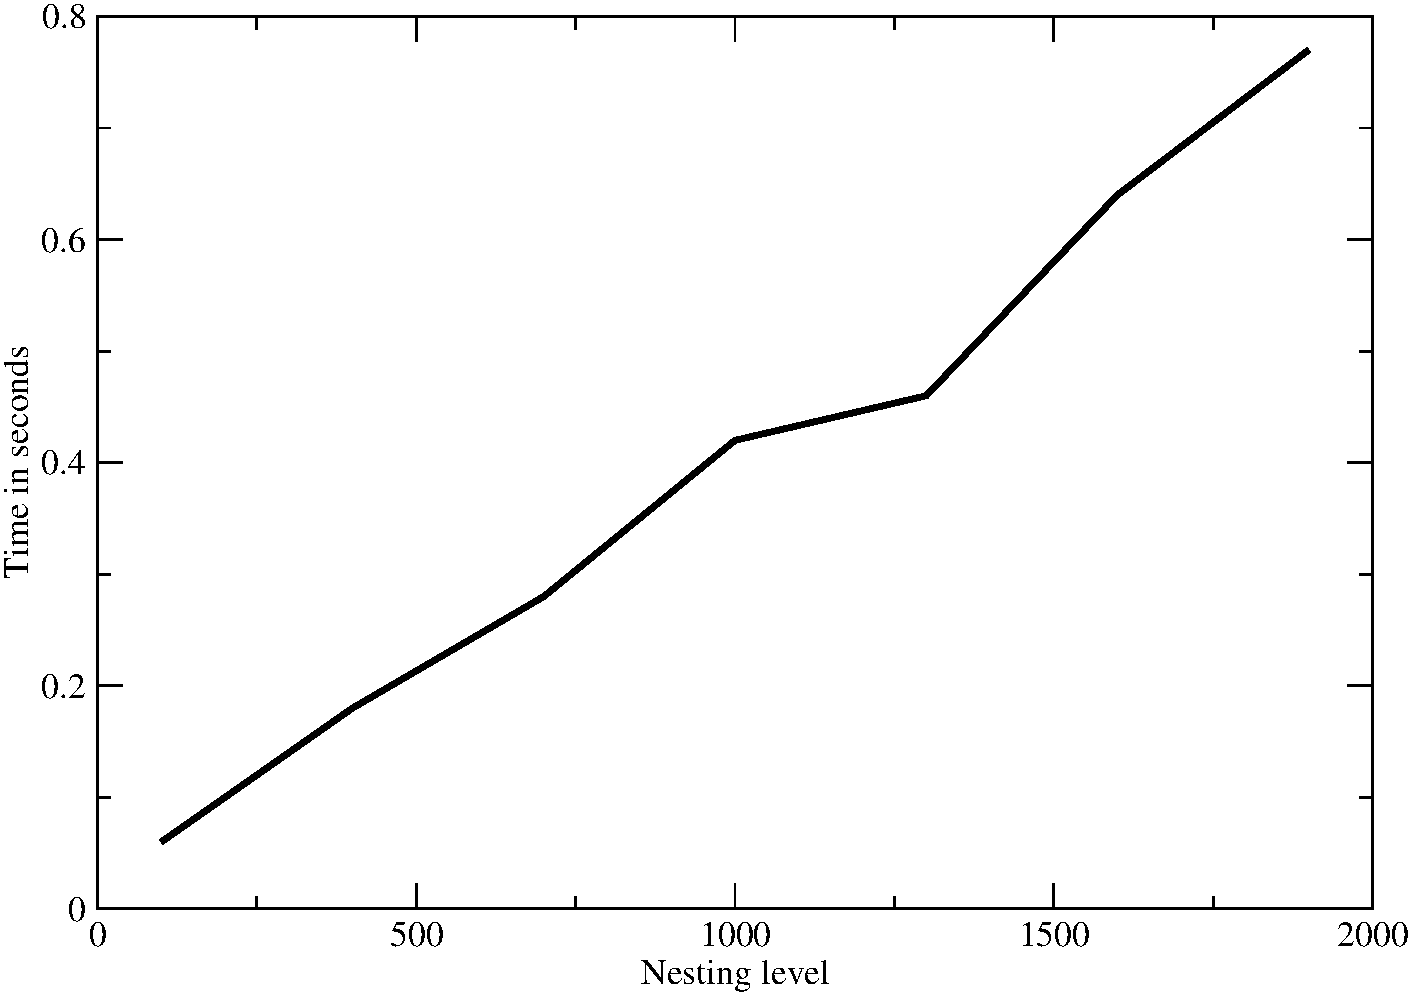
\includegraphics[width=0.95\columnwidth]{figs/nesting.pdf}
\begin{minipage}{0.95\columnwidth}
  \caption{\label{fig:nesting} Relationship between nesting depth and runtime in nested if example.}
\end{minipage}
\end{center}
\end{figure}

The second experiment we ran with the nested if generator was intended
to show that varying the structure of the graph given a constant node
and edge count has a significant impact runtime. In this experiment,
we held the node count fixed at 4000 and varied the depth of the
nested if blocks. Figure~\ref{fig:nesting} shows the result. We find
that runtime varies linearly with the depth of nesting. This shows
that for the dominance algorithm we implemented, it is insufficient to
describe its performance only in terms of nodes and edges---the
structure of the CFG has a significant effect on its performance.

\section{Conclusion}

We implemented a dominance algorithm for the Start intermediate
language. We found that the algorithm performs well for our example
programs, and that the structure of the CFG has a significant effect
on the performance of domincance detection.

\bibliographystyle{abbrv}
\bibliography{writeup}

\end{document}

